\section{Convolution and Image Transforms}

As seen in Chapters \ref{chapter:fundamentals-of-optics-and-light-microscopy} and \ref{chapter:blur-characterization-and-image-formation}, the processes of image formation and acquisition concerning linear systems are subject to some operations, i.e. the convolution, the \sigla{FT}{Fourier Transform} and its continuous and discrete versions, that modify the original representation of the scene. The linear system theory provides mathematical tools to explore these operations and others, such as sampling, filtering, and enhancement; it describes the behavior of electrical circuits and optical systems \cite{castleman1996digital}.

According to \citeonline{bracewell2000fourier}, the convolution of two arbitrary functions $s$ and $t$ that results in another function $r$ is, with notation adjustments, defined by the integral

\begin{equation}
\label{eqn:one_dimensional_convolution}
r(x) = \int_{-\infty}^{\infty}s(u) t(x - u) du,
\end{equation}

\noindent where $x$ is the one-dimensional coordinate and $u$ is a shifting parameter. In other words, this procedure is compared to moving a 180 degree-rotated filter mask over the function values and computing the sum of products at each location \cite{gonzalez2018digital}. Hence, the shifting parameter represents the slide of the filter mask over the values. As seen in \autoref{chapter:blur-characterization-and-image-formation}, convolution is responsible for the image formation and acquisition processes, but it also covers several other applications, e.g. smoothing, sharpening and reducing noise in images. Similarly to the one-dimensional case and pursuant to \citeonline{castleman1996digital}, the two-dimensional convolution is denoted by

\begin{equation}
\label{eqn:two_dimensional_convolution}
r(x,y) = \int_{-\infty}^{\infty}
         \int_{-\infty}^{\infty}
         s(u,v) t(x - u, y - v) du dv,
\end{equation}

\noindent where $u$ and $v$ are shifting parameters, and $\ast$ denotes the convolution. The \emph{spatial domain} is the subset of the real plane where functions like $r$, $s$ and $t$ are spanned, and $(x,y)$ as points within such subset are named spatial variables; consequently, any mathematical operation that employs pixels from this subset is named a spatial domain technique. As for the digital image processing applications, which deal with images as matrices of pixels, the discrete two-dimensional convolution for an image $f(x,y)$ and a function $h(x,y)$ is given by 

\begin{equation}
\label{eqn:2d_discrete_convolution}
g(x,y) = h(x,y) \ast f(x,y) = 
        \sum_{m=-a}^{a}
        \sum_{n=-b}^{b}
        f(m,n) h(x-m,y-n),
\end{equation}

\noindent where $a = (m-1)/2$ and $b = (n-1)/2$, given that the function $h(x,y)$ is considered to be a two-dimensional filter of size $m \times n$ \cite{gonzalez2018digital}.

Convolution, together with several other operations employed in this work, operate directly on the spatial domain by modifying pixel values based on mathematical constraints. Some of those operations may have issues that hinder the operation, e.g. the computation time of a convolution process should be finite, otherwise, its use is impractical; this is one of the reasons why \emph{image transforms} are widely used. They encompass any group of mathematical operations that transfers the input signal or image from its domain to the transform domain \cite{gonzalez2008digital}. Let $s$ be an arbitrary two-variable function, $t_{f}$ and $t_{i}$ be the forward and inverse transformation kernels, respectively. The general discrete form of the forward and inverse two-dimensional transforms is denoted by 

\begin{align}
\label{eqn:generic_transform}
R(u,v) = 
\sum_{x=0}^{M-1}
\sum_{y=0}^{N-1}s(x,y)t_{f}(x,y,u,v)
&&
s(x,y) = 
\sum_{x=0}^{M-1}
\sum_{y=0}^{N-1}R(u,v)t_{i}(x,y,u,v),
\end{align}

\noindent where $M$ and $N$ are the dimensions of the image, $x$ and $y$ are coordinates of the image, $u = \{0,1,2,...,M-1\}$ and $v = \{0,1,2,...,N-1\}$ are called transform variables. The $t_{f}$ function is responsible for the forward domain change and the $t_{i}$ transfers the image back to the spatial domain. Switching from spatial to frequency domain, for example, allows different operations to be executed that otherwise could not be performed in the spatial domain. The convolution operation, for instance, turns itself into a simple matrix multiplication task on the Fourier Transform domain (which will be detailed in the following sections) and that solves the performance constraint.

\section{Image Enhancement}

Image enhancement is the process of manipulating an image in order to provide a resulting representation that is more suitable for a particular problem, e.g. an enhancement method for medical images may not be efficient for satellite images \cite{gonzalez2018digital}. In microscopy, image enhancement is desirable due to the limited capacity of optical imaging devices and the drawbacks posed by each microscopy technique, e.g. acquisition with different illumination settings, focal planes, time intervals or spectral channels. Therefore, enhancement algorithms for microscopy should cover all types of information \cite{wu2008microscope}. According to \citeonline{wu2008microscope}, image enhancement techniques are divided into \emph{spatial domain}, \emph{Fourier transform} and \emph{wavelet transform} methods. They will be described in the following paragraphs. 

The spatial domain methods are transforms that work directly on pixels of the image \cite{gonzalez2018digital}. Some examples are contrast stretching (redistribution of image gray levels to a wider range), thresholding (image binarization given a preset gray level), histogram equalization, and spatial filtering. Particularly, histogram equalization and spatial filtering play an important role in this work and therefore will be explored further.

Fourier transform domain methods operate with images as a distribution of frequencies since some features are better described by it. Noise, for example, may be suppressed in a sharpening process or reduced by amplifying mid-frequency components and attenuating high-frequency ones. The Wiener Filtering process is a popular example of a frequency domain enhancement method that recovers a noisy signal or image based on estimations of spectral properties from the original image. Other examples of Fourier domain enhancement are band-pass filters and least-squares deconvolution applications. 

Finally, there are methods based on the Wavelet Transform, i.e. a mathematical framework that decomposes images or signals into frequency components in different scales. Some operations such as thresholding may be applied to wavelet coefficients. However, the output of the wavelet transform is not always the same; it depends on the chosen wavelet function and consequently should be properly set in order to extract the desired image features.

The image histogram is one of the simplest and most useful tools in image processing and consists of a function that summarizes the gray level content of an image in terms of a frequency distribution \cite{castleman1996digital}. The histogram equalization consists of a non-linear monotonic mapping to provide an approximation of a uniform distribution to the output image's histogram \cite{gonzalez2018digital}. The output histogram is a normalization of the cumulative histogram of the image, given by

\begin{equation}
\label{eqn:histogram_equalization}
hist_{equalized}(r) = \frac{L - 1}{MN} hist_{cumulative}(r),
\end{equation}

\noindent where $hist_{equalized}(r)$ and $hist_{cumulative}(r)$ are the equalized and cumulative histograms relative to a range $L$ of intensities after the image quantization with $r$ values. $M \times N$ is the image resolution. Since it stems from a sum of probabilities and no new gray intensity levels should be created, the process generates fractional values that are mapped onto integers.

Spatial filtering consists of the convolution of an image with a predefined kernel operator \cite{gonzalez2018digital}. The continuous form may be represented as a convolution over all values of a defined region of the image and the discrete form consists of sliding a weight mask over the image \cite{wu2008microscope}. \autoref{fig:generic_spatial_filtering} presents an arbitrary schema of a simple linear spatial filtering procedure:

\begin{figure}[htb]
	\centering
	\caption{\label{fig:generic_spatial_filtering} Arbitrary example of linear spatial filtering of an image (a) with a $3 \times 3$ filter mask (b), which results in filtered sections (c).} 
	\begin{center}
	    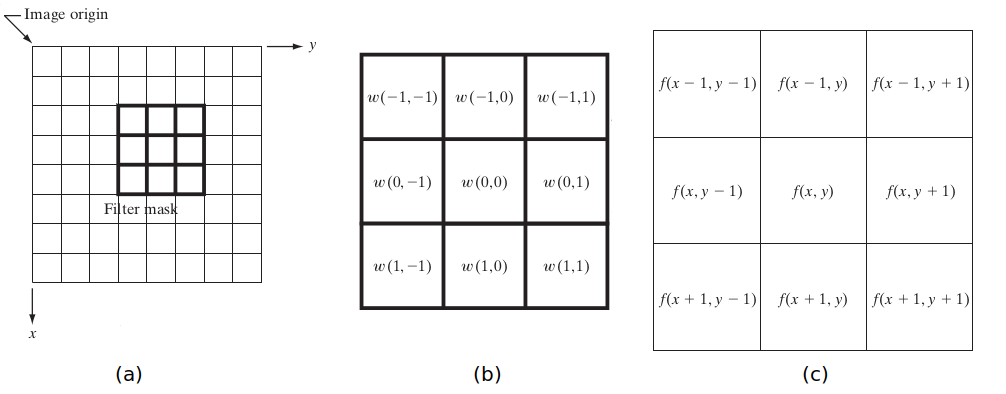
\includegraphics[scale=0.4]{images/generic_spatial_filtering.png}
	\end{center}
	\centering
    \fadaptada{gonzalez2018digital}
\end{figure}

Examples of discrete spatial filtering in digital image processing are smoothing filters, order-statistic nonlinear filters and sharpening filters \cite{gonzalez2018digital}. Spatial smoothing filters are applied to remove details, edges and lines from an image to reduce noise. The order-statistic nonlinear filters are based on ordering pixels of the image under the filter area and replacing the pixel value in the center of the area with the response from ordering; one example is the \emph{median filter}, which replaces the center pixel with the median of pixels in its neighborhood. Median filters yield significant noise reduction effects if the nature of the noise is random. Finally, the sharpening filters are built to highlight transitions in intensity by spatial differentiation and are used for enhancing edges.

\section{Image Registration}

When images belonging to the same scene are acquired in different conditions such as distinct focus configurations, sensors, or even at different times, they should be geometrically aligned according to a reference image. The process of overlaying two or more images with different acquisition settings is named image registration and plays an important role as a pre-processing step for image fusion, change detection and multichannel image restoration \cite{zitova2003image}. According to \citeonline{gonzalez2018digital}, magnetic resonance imaging and positron emission tomography systems, for example, are two different medical image modalities that may require images to be registered. Images which were taken in different times such as satellite images also need to be registered.

The image registration methods consist of the following steps, as reported by \citeonline{zitova2003image} and \citeonline{gonzalez2018digital}:

\begin{itemize}
    \item \emph{Feature detection}: manually or automatically detect distinctive objects, e.g. edges, contours, corners and represent those as \emph{control points}, i.e. points with known locations in the reference and input images;

    \item \emph{Feature matching}: a relationship between the detected features in each image is established using feature descriptors;

    \item \emph{Transform model estimation}: parameter estimation for mapping functions that align the input images with the reference image, either by establishing feature correspondence or performing an optimization procedure;

    \item \emph{Image resampling and transformation}: the image is resampled with interpolation techniques.

\end{itemize}

Image registration is, in practice, a mapping between two or more images by means of a spatial and an intensity transformation \cite{brown1992survey}. Some prominent examples of registration methods are the principal axes, multiresolution, optimization-based, boundary, model-based and adaptive methods  \cite{goshtasby2012image}. The spatial transformations play an important role in all image registration techniques, and the most common examples are rigid, affine, projective, perspective and global polynomial \cite{brown1992survey}. Also pursuant to \citeonline{brown1992survey}, each of such transformations may be described as:

\begin{itemize}
    \item \emph{Rigid}: accounts for object or sensor movement in which objects in the images retain their relative shape and size. Example: \emph{rigid-body transformation} which combines rotation, translation and scale changes; 
    
    \item \emph{Affine}: handle more complicated distortions and preserve mathematical properties. Example: \emph{shear transformation};
    
    \item \emph{Projective and Perspective}: the former deals with distortions due to projection of the objects at varying distances to the sensor onto the image plane, and the latter demands prior knowledge about the locations of the objects in the scene relative to the sensor;
    
    \item \emph{Polynomial}: cover the broadest range of distortions, as long as they are approximately homogeneous in the image.
\end{itemize}

\section{Image Fusion}
Image fusion is a process that merges several images, possibly acquired in diverse conditions or with different cameras, into one image with higher quality, more details and consequently more useful for humans and computer tasks \cite{mitchell2010image}. Examples of image fusion applications are noise reduction, edge enhancement, and super-resolution. One traditional use of image fusion occurs in medical imaging fields; the quality of information about illnesses, cells, clinical analysis and several other medical tasks (including the computer-assisted ones) have found profitable results from the image fusion techniques and led themselves to better and faster decisions when it comes to human beings \cite{james2014medical}. There are also relevant applications in remote sensing multispectral images, segmentation of regions in different color spaces, biometry: the pan-sharpening process is the generation of a high-resolution multispectral image from low to high-resolution ones, K-Means segmentation and fusion of pixels in the RGB and the Iris Recognition biometric process with video frames are examples of such tasks, respectively \cite{mitchell2010image}.


Also according to \citeonline{mitchell2010image}, the general framework for the image fusion procedure consists of four stages: \emph{Multiple Input Images}, \emph{Common Representational Format}, \emph{Fusion} and \emph{Display}.
The multiple input images stage is simply the acquisition of the images to be merged. There are several approaches to this: the dataset may be captured from different sensors, under distinct light conditions or angles, with different magnifications, under several focus settings, and with temporal measurements, if the scene changes through time.

If the acquired dataset images do not share the same features such as dimension, rotation angle, and resolution, then the images should be pre-processed in order to arrive at a common state. This configures the common representational format step, which generates a new and temporary dataset with the same properties, e.g. color space, dimensions, and noise level. The fusion stage employs a decision method to dictate which regions, objects, colors or details will compose the final image; some methods rely on the wavelet transform, for example. Finally, the display stage provides a view of the resulting image, which can be used directly for any further task or even be the input for other image processing operations. \autoref{fig:fusion_general_framework} depicts an arbitrary example of the four stages. 

\begin{figure}[ht]
	\centering
	\caption{\label{fig:fusion_general_framework}Image fusion general framework. (a) Multiple Input Images, (b) Common Representational Format, (c) Fusion and (d) Display.}
	\begin{center}
    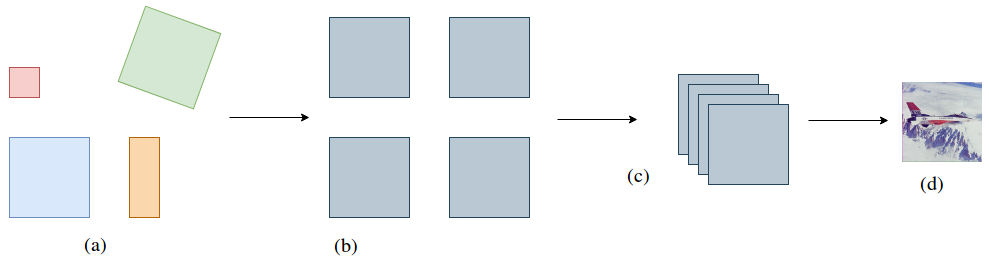
\includegraphics[scale=0.45, trim={0 -1.5cm 0cm -1.5cm}, clip]{images/image_fusion_scheme.png}
	\end{center}
	\centering
    \fautor
\end{figure}

The four arbitrary images in \autoref{fig:fusion_general_framework}.\textbf{(a)} represent different images of the same scene, taken at different resolutions, rotation angles, and shapes. In \autoref{fig:fusion_general_framework}.\textbf{(b)}, the images are all reshaped, converted to common color space and ready to undergo the processing algorithm which will transform them into feature vectors. \autoref{fig:fusion_general_framework}.\textbf{(c)} represents the image fusion by means of an arbitrary fusion rule. The resulting image is depicted in \autoref{fig:fusion_general_framework}.\textbf{(d)}. Since image fusion is only one branch of data fusion field, this procedure has a wide variety of approaches and methods; hence, the domain will be restricted to the multi-focus image fusion and some relevant related work will be presented in \autoref{chapter:related-work}.

\section{Image Quality Assessment}
\sigla{IQA}{Image Quality Assessment} is the evaluation of image quality as perceived by an average human observer, i.e. how close an image is to a given original or reference image. It is also related to the accuracy of the image acquisition process for an imaging system \cite{bovik2009essential}. It is known that images are frequently used in health and life sciences, public security systems, remote sensing, and several other fields; hence, there are computational applications that offer some useful service employing image processing. As a result, assessing image quality poses as an important task among those applications for which several techniques are being developed, evolved and deployed.

According to \citeonline{tang2019feature}, the IQA methods are distributed between the subjective assessment and objective assessment categories. The former is based on a well-defined test environment for random observers to label images and provide the final \sigla{MOS}{Mean Opinion Scores}, while the latter is based on the use of strategies such as statistical modeling, machine learning, spatial or spectral image features and so on. It is evident that subjective IQA is demanding; consequently, objective methods are preferred to conduct IQA.

According to \citeonline{wang2004image}, there are three classes of objective image quality metrics that relate to the existence of a no-distortion image (or with a negligible amount of it) for comparison purposes. The \sigla{FR-IQA}{Full-Reference Image Quality Assessment} methods assume that the reference image is available, while \sigla{RR-IQA}{Reduced-Reference Image Quality Assessment} methods employ a representation of the reference image, such as a set of extracted features. Finally, the \sigla{NR-IQA}{No-Reference Image Quality Assessment} methods, also known as ``blind'', are those which do not employ a reference image. \autoref{fig:mssim_IQA_exampe} denotes an example of a full-reference method, the \sigla{MSSIM}{Mean Structural Similarity Measure} method and its output for an image with different types of degradation:

\begin{figure}[ht]
	\centering
	\caption{\label{fig:mssim_IQA_exampe} Example of the MSSIM method output: Original image (a), contrast-stretched image (b), mean-shifted image (c), JPEG compressed image (d), blurred image (e) and salt-pepper impulsive noisy image (f).}
	\begin{center}
    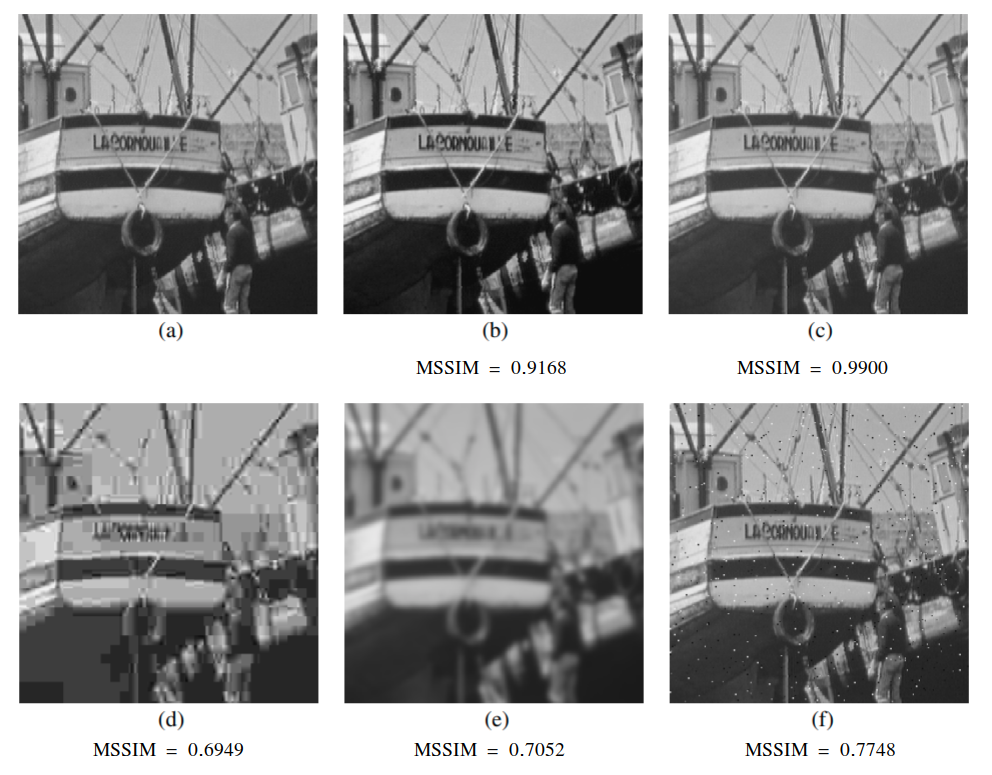
\includegraphics[scale=0.4]{images/mssim_IQA.png}
	\end{center}
	\centering
    \fdireta{wang2004image}
\end{figure}

IQA methods are also present within microscopy and its close interaction with image processing. The image acquisition in microscopy techniques may involve lasers, transmitted or reflected light, measurements of atomic force responses, the fluorescence of chemical compounds and several other means. Each technique has an inherent kind of degradation that affects the acquired images or spectra, e.g. the Raman confocal microspectroscopy suffers from the interference of cosmic rays, which yields unexpected peaks in the spectrum. Therefore, the use of IQA methods is expected. They will be investigated and used in this work. In \autoref{chapter:related-work}, some examples of NR-IQA techniques that guided the development of our method will be presented.

\section{Statistics}

Statistics is the science of planning studies and experiments, obtaining, organizing, summarizing, presenting, analyzing, and interpreting data and finally drawing conclusions. \emph{Descriptive statistics} is an important branch that comprises a set of methods which aim to describe relevant characteristics in data \cite{triola2017elementary}. The descriptive statistics methods either employ graphical elements such as boxplots, histograms, bar graphs and scatter plots to analyze data or yield numerical summary measures such as means, standard deviations, correlation coefficients and other related indices \cite{devore2011probability}. The methods that compose a descriptive statistical approach for data analysis are simple yet powerful tools.

The concepts of \emph{population}, \emph{sample} and \emph{variable} are elementary: a population is a well-defined collection of objects that might be included in the analysis, a sample is a subset of a population and a variable is a feature of the objects which may change from one object to another \cite{devore2011probability}. Moreover, a \emph{frequency distribution} is a tool that presents how the data is partitioned among several categories by listing each category and its frequency of data values; a \emph{relative frequency distribution} is a frequency distribution in which each frequency is represented by a proportion, usually as percentage \cite{triola2017elementary}. According to \citeonline{mendenhall2016statistics}, the measures of central tendency provides several ways to locate the center of the relative frequency distribution, and the three most common are the \emph{arithmetic mean}, i.e. the average of the measurements, the \emph{median}, i.e. the middle number when the measurements are ordered in ascending or descending order and the \emph{mode}, i.e. the value that occurs with the greatest frequency. Mathematically, the arithmetic mean is given by

\begin{equation}
\label{eqn:arithmetic_mean}
\bar{x} = \frac{1}{n} \sum_{i=1}^{n} x_{i} = \frac{x_{1} + x_{2} + \dots + x_{n}}{n},
\end{equation}

\noindent where $n$ is the sample size and $x_{i}$ represents the $i$-th observation of the variable $x$ \cite{zwillinger1999crc}.

% \subsection{Measures of Variation}

The measures of variation provide a description of how the values spread along the distribution. Commonly used measures are the range, the variance, and the standard deviation \cite{mendenhall2016statistics}. The range is simply the difference between the largest and the smallest value within the data, which may precisely point out its variability, since it does not comprise the middle values among the distribution \cite{devore2011probability}. The variance and the standard deviation are closely related, as the former measures variability based on the squared deviations about
the mean and the latter is the positive square root of the variance, as

\begin{align}
\label{eqn:variance_std}
\sigma^{2} = \frac{1}{n - 1} \sum_{i = 1}^{n} \left(x_{i} - \bar{x}\right)^{2}
&&
\sigma = \sqrt{\sigma^{2}}
\end{align}

\noindent where $\sigma^{2}$ and $\sigma$ are respectively the variance and the standard deviation, $x_{i}$ is the $i$-th observation of the variable $x$, $\bar{x}$ is the mean, all concerning a sample or the population \cite{zwillinger1999crc}.

% \subsection{Measures of Relative Standing and Outlier Detection}

The measures of the relative standing of an observation describe its location among other values in the distribution, and two examples of these measures are \emph{percentiles} and \emph{z-scores}; also, an observation located outside the range of the distribution is an \emph{outlier} \cite{mendenhall2016statistics}. Percentiles are values that split the data into 100 parts in a sorted dataset, so that the $i$-th percentile stands for the $i(n + 1) / 100$ observation, e.g. the $25$-th percentile comprises $25\%$ of the data; the $z$-score, or standard score, is given by

\begin{equation}
\label{eqn:z_score}
z = \frac{x_{i} - \bar{x}}{\sigma},
\end{equation}

\noindent where $x_{i}$ is the $i$-th observation of the variable $x$, $\bar{x}$ is the mean and $\sigma$ is the standard deviation of the population or the sample \cite{zwillinger1999crc}. 

The Interquartile Range (IQR) is the length of the interval that contains the middle half of the distribution \cite{degroot2012probability}. Mathematically, it is the difference between the third ($Q_{3}$) and the first ($Q_{1}$) quartiles, i.e. the $75$th percentile $25$th percentile, respectively \cite{devore2011probability}. The IQR is described by

\begin{equation}
\label{eqn:iqr}
IQR = Q_{3} - Q_{1}.
\end{equation}

% \subsection{Probability Distributions}

Probability is a common and natural concept among human life, used in expressions such as ``It probably will be cold tonight''; however, there is no common formal definition accepted among statisticians and related researchers \cite{degroot2012probability}. The study of randomness, variability and uncertainty in populations is done by analyzing probabilities, i.e. numerical descriptions of how likely an event is to occur \cite{devore2011probability}. Some basic concepts that support the probability theory are described also to the light of \citeonline{devore2011probability}, as follows:

\begin{itemize}
    \item \emph{Experiment}: any activity or process whose outcome is subject to uncertainty;
    
    \item \emph{Sample Space}: the sample space of an experiment is the set of all possible outcomes for it;
    
    \item \emph{Event}: any collection or subset of outcomes of a sample space;
    
    \item \emph{Random Variable}: any rule that associates a number with each outcome in a sample space of some experiment; mathematically, it is a function with the sample space as its domain and the real numbers as its range;
    
    \item \emph{Discrete Random Variable}: a random variable with a finite set or a countable infinite sequence of possible values;
    
    \item \emph{Continuous Random Variable}: a random variable that yields zero as the probability for every possible outcome or its set of possible values are in a single interval of the real line or all numbers in a disjoint union of intervals.
    
\end{itemize}

From these concepts, it is possible to define a distribution in the scope of the probability theory. The \emph{probability distribution} is a collection of all probabilities computed from a  discrete or continuous random variable with the set of real numbers; a \emph{discrete} probability distribution is represented by the probability function itself, while a \emph{continuous} probability distribution is represented by a \sigla{p.d.f}{probability density function} \cite{mendenhall2016statistics}.


The \emph{kurtosis} is one of the probability distribution shape statistics, which measures the extent of the peak in a distribution, i.e. its ``peakedness''; smaller absolute values indicate that the distribution tends to be uniform \cite{zwillinger1999crc}. First of all, the concepts of \emph{expectation} and \emph{moments} should be described. The expectation of a random variable (and consequently, of a distribution) is a value that summarizes its nature and is given by

\begin{align}
\label{eqn:expectation}
E(X) = \int_{-\infty}^{\infty} x p(x)dx
&&
E(X) = \sum_{x} x p(x),
\end{align}

\noindent where $x$ is each possible outcome of the random variable $X$, $p(x)$ is the probability density function for a continuous random variable (left) and the probability function for a discrete random variable (right) \cite{degroot2012probability}. Still according to \citeonline{degroot2012probability}, for a random variable $X$ and every positive $k \in \mathbb{R}$, the expectation $E(X^{k})$ is
called the $k$-th moment of $X$. The $r$-th moment may be described, according to \citeonline{zwillinger1999crc}, as

\begin{equation}
\label{eqn:rth_moment}
m_{r} = \frac{1}{n}
        \sum_{i=1}^{k}p_{i}(x_{i} - \bar{x})^{r}
\end{equation}

\noindent for every $x_{i}$ in the possible outcomes of $X$. Thus, kurtosis may be defined as the ratio of the fourth moment (\autoref{eqn:rth_moment} with $r = 4$) by the square of the variance (also \autoref{eqn:rth_moment} with $r = 2$), denoted by

\begin{equation}
\label{eqn:kurtosis}
g_{2} = \frac{m_{4}}{(m_{2})^{2}} - 3
\end{equation}

The $-3$ constant is inherited from Fischer's approach, where the kurtosis of a normal distribution is zero.